\section{Method}
\label{sec:method}

\subsection{Problem Formulation and GRPO}
\label{sec:problem_formulation}

We model the multi-turn agent as a partially observable Markov decision process (POMDP)~\citep{kaelbling1998planning} where the policy $\pi_\phi(a_t \mid h_t)$ generates actions conditioned on interaction history $h_t = (o_1, a_1, \ldots, o_t)$. Episodes of $T$ steps terminate with binary reward $R \in \{0, r_+\}$ (our experiments use a penalty variant with $r_- = -0.1$ per invalid action; Section~\ref{sec:setup}). GRPO~\citep{shao2024deepseekmath} samples $K$ rollouts per task and computes group-relative advantages:
\begin{align}
\hat{A}_k &= \frac{R_k - \mu}{\sigma + \epsilon}, \notag \\
\mu &= \frac{1}{K}\sum_{j=1}^K R_j, \quad \sigma = \sqrt{\frac{1}{K}\sum_{j=1}^K (R_j - \mu)^2}
\label{eq:grpo_advantage}
\end{align}
GRPO is episode-level by design: each rollout receives one return and one advantage, with no inherent temporal discounting.

\subsection{Step-Independent Windowing}
\label{sec:step_independent}

Agent RL frameworks must reconcile GRPO's episode-level design with the memory constraints of long trajectories. RAGEN~\citep{ragen2025} introduces \textbf{step-independent training}: the trajectory is partitioned into non-overlapping $h$-step windows, each receiving a discounted return:
\begin{equation}
R_w = \gamma^{(N - w)} \cdot R_{\text{episode}}
\label{eq:step_return}
\end{equation}
where $w \in \{1, \ldots, N\}$ indexes windows and $N = \lceil T/h \rceil$ is the number of windows. Each window is optimized as an independent GRPO sample. This reduces sequence length from $O(T)$ to $O(h)$ and multiplies the effective batch size, but structurally alters credit assignment.

\subsection{Dual Mechanism Analysis}
\label{sec:dual_mechanism}

Two mechanisms jointly cause training failure under step-independent optimization.

\subsubsection{Mechanism 1: Policy Information Loss}
\label{sec:m1_information_loss}

Step-independent training truncates context at both inference and training time. The policy $\pi_\phi(a_t \mid h_{\text{window}_w})$ conditions on only the local $h$-step history, losing access to earlier observations. With $h{=}2$, a window at step~8 has no access to the outcome of an exploration action at step~4, so the policy cannot learn strategies spanning more than $h$ steps. This imposes a \textit{constant} performance ceiling: no amount of optimization can recover absent information.

\subsubsection{Mechanism 2: Advantage Sign Misattribution}
\label{sec:m2_sign_misattribution}

Group normalization under step-independent training produces advantages whose sign reflects the \textit{episode} outcome, not local action quality:
\begin{equation}
\text{sign}(\hat{A}_w) \approx \text{sign}(R_{\text{episode}} - \mu)
\label{eq:sign_correlation}
\end{equation}
In failed episodes ($R_{\text{episode}} = 0$), all windows receive negative advantages when $\mu > 0$, including windows with locally correct actions. Conversely, successful episodes reinforce all windows, including those with suboptimal actions. Unlike M1's constant ceiling, sign misattribution is \textit{cumulative}: each wrong-sign gradient step further erodes policy competence. The discount factor $\gamma^{(N-w)}$ introduces magnitude decay across positions, but sign errors are strictly more harmful: magnitude decay slows convergence, while sign errors cause active divergence.

\subsection{Episode-Level Training}
\label{sec:episode_level}

Episode-level training structurally eliminates both mechanisms by treating the complete trajectory as a single GRPO sample. The full history $h_t$ is available at every step (eliminating M1), and a single advantage $\hat{A}$ applies uniformly to all tokens (eliminating M2). Uniform reinforcement of successful trajectories preserves good sub-strategies; window-level sign errors actively destroy them. This restores GRPO's original per-sample granularity to the episode level; step-independent windowing is the deviation introduced by multi-turn agent frameworks.

\subsection{Partial Factorial Design}
\label{sec:factorial_design}

To separate the two mechanisms, we design a $2 \times 2$ partial factorial varying observation scope and advantage granularity: \textbf{Cell~A} (truncated $h{=}2$ + step-level advantage; both mechanisms active), \textbf{Cell~B} (truncated $h{=}2$ + episode-level advantage; only M1 active), \textbf{Cell~D} (full trajectory + episode-level advantage; neither active), and \textbf{Cell~C} (full trajectory + step-level advantage; only M2 active). Cell~C encountered persistent numerical instability across six hyperparameter configurations (Appendix~\ref{app:cell_c}); we therefore evaluate a partial 3-of-4 factorial. Comparing A vs.\ B isolates sign misattribution; comparing B vs.\ D isolates information loss.

\begin{figure*}[t]
\centering
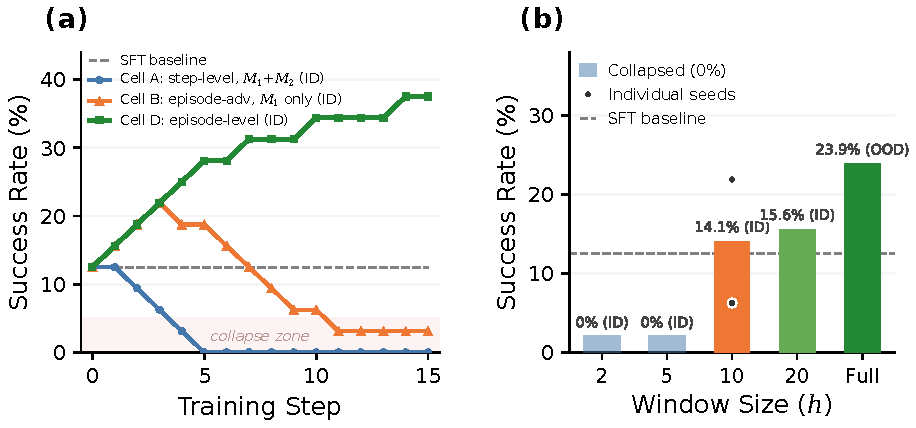
\includegraphics[width=\textwidth]{fig_training_dynamics.pdf}
\caption{(a)~Training dynamics across partial factorial conditions. Cell~A collapses; Cell~B shows bounded learning; Cell~D improves monotonically. (b)~Window size $h$ vs.\ success rate. Bars show mean over available seeds; black dots at $h{=}10$ show individual seeds (2 seeds), revealing seed-dependent instability at this boundary. Hatched bars indicate collapsed conditions ($0\%$).}
\label{fig:hsweep}
\end{figure*}
